\documentclass[a4paper,11pt]{article}
\usepackage[T1]{fontenc}
\usepackage[utf8]{inputenc}
\usepackage{lmodern}
\usepackage{graphicx}
\usepackage{subcaption}

\title{Reinforcement Learning results analysis}
\author{Marco Marini}

\begin{document}

\maketitle
\tableofcontents

\begin{abstract}
Reinforcement Learning results analysis.
\end{abstract}

\section{Measure}

One hundred tests were run a maze environment with two different $\lambda$ values.

Each test consist of 1000 episodes with a limit of 300 steps per episode.

\section{TDQAgent}

The returns of TDQAgent slightly increase from about -565 to -555 while the optimal value should be about -4.

The agent was not able to learn the optimal strategy due to probable the impossibility to find the path within limit of 300 steps.

The errors increase from 6 to about 3000. The cause of such increment may be due to boostrap effect.
No optimal and stable policy was found and so the action values decrease incrementally without a lower bound limit.
The changes of network parameters do not fit such limits createing incremental errors episode by episodes.

No significant differences of learning rate can be noted changing the hyper parameter $\lambda$.

\begin{figure}[h!]
	\centering
	\begin{subfigure}[b]{0.4\linewidth}
		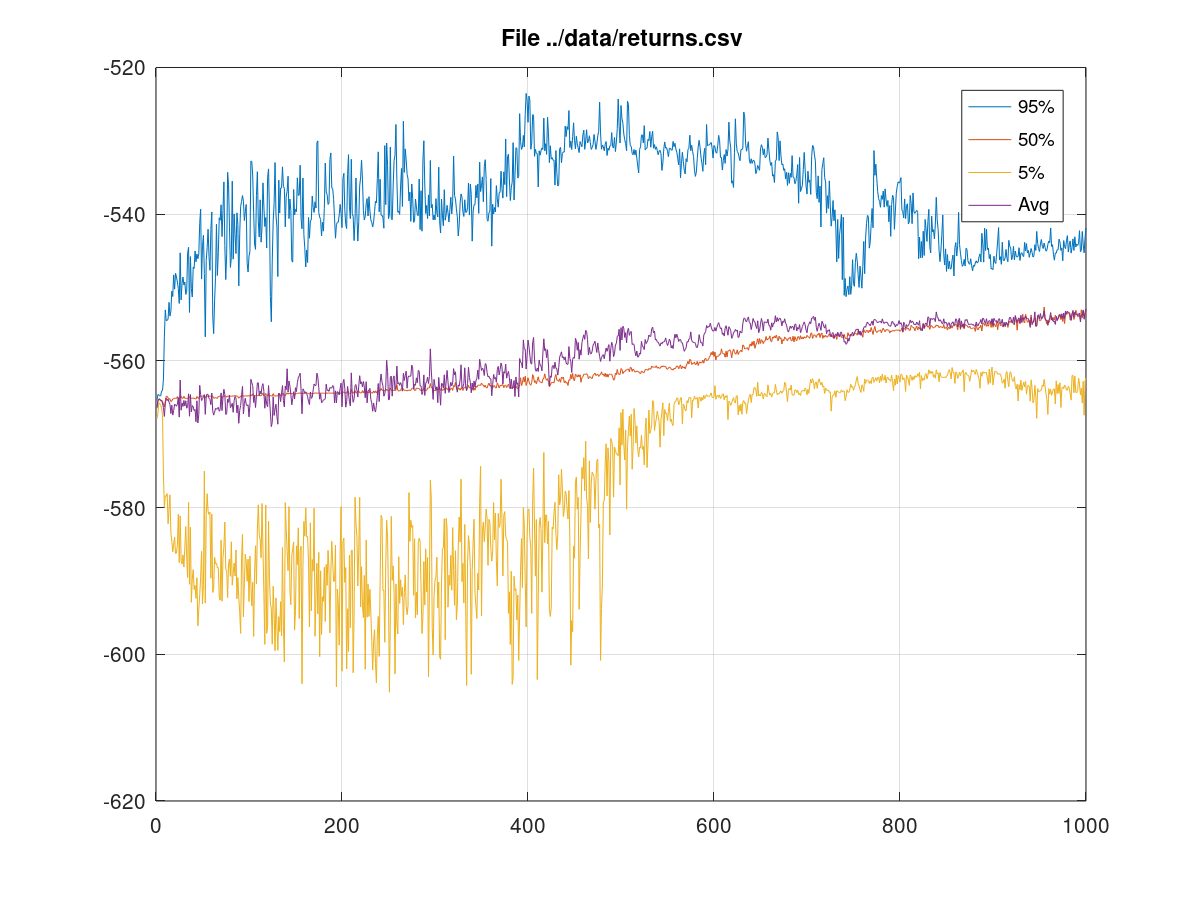
\includegraphics[width=\linewidth]{returns-0.png}
		\caption{$\lambda=0$.}
	\end{subfigure}
	\begin{subfigure}[b]{0.4\linewidth}
		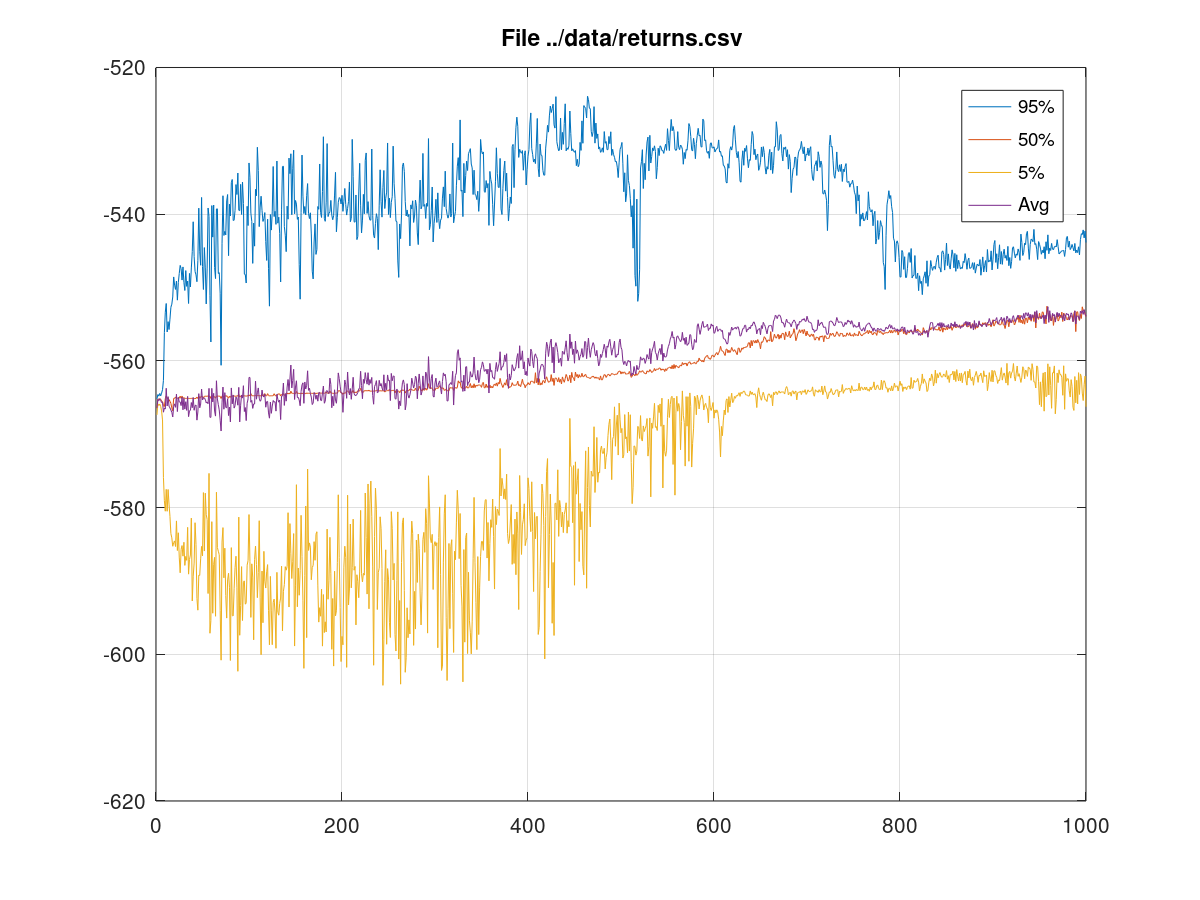
\includegraphics[width=\linewidth]{returns-07.png}
		\caption{$\lambda=0.7$.}
	\end{subfigure}
	\caption{Returns}
	\label{fig:returns}
\end{figure}

\begin{figure}[h!]
	\centering
	\begin{subfigure}[b]{0.4\linewidth}
		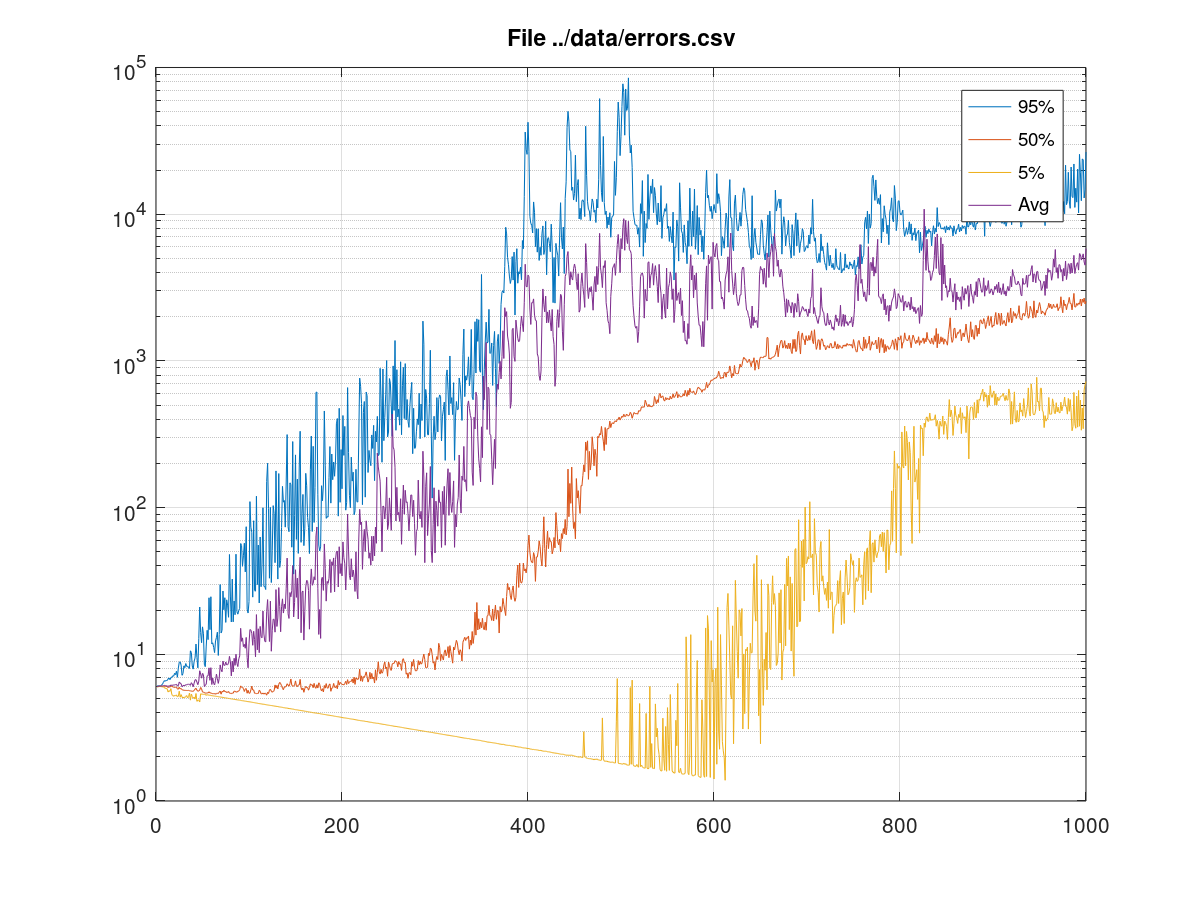
\includegraphics[width=\linewidth]{errors-0.png}
		\caption{$\lambda=0$.}
	\end{subfigure}
	\begin{subfigure}[b]{0.4\linewidth}
		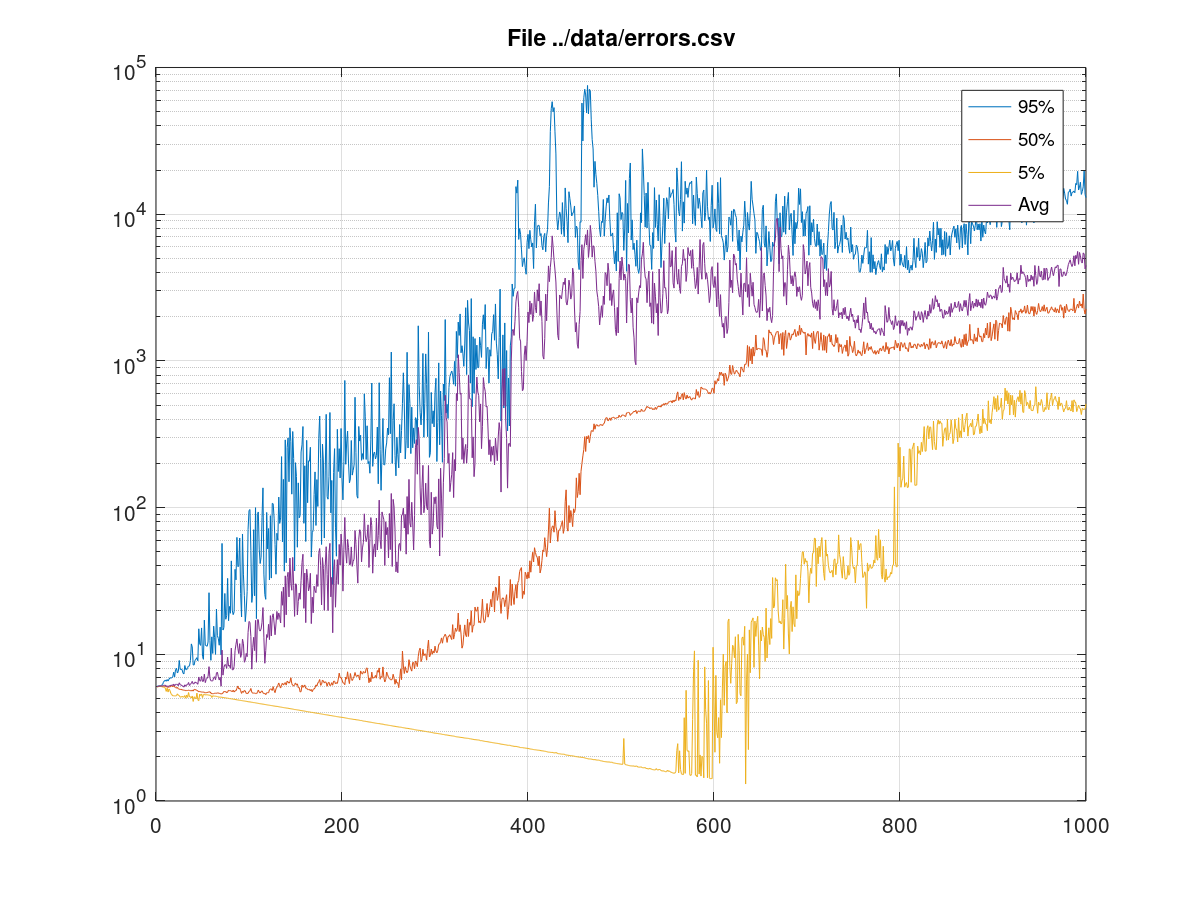
\includegraphics[width=\linewidth]{errors-07.png}
		\caption{$\lambda=0.7$.}
	\end{subfigure}
	\caption{Errors}
	\label{fig:errors}
\end{figure}

\section{Adam}

The figure {}
\begin{figure}[h!]
	\centering
	\begin{subfigure}[b]{0.4\linewidth}
		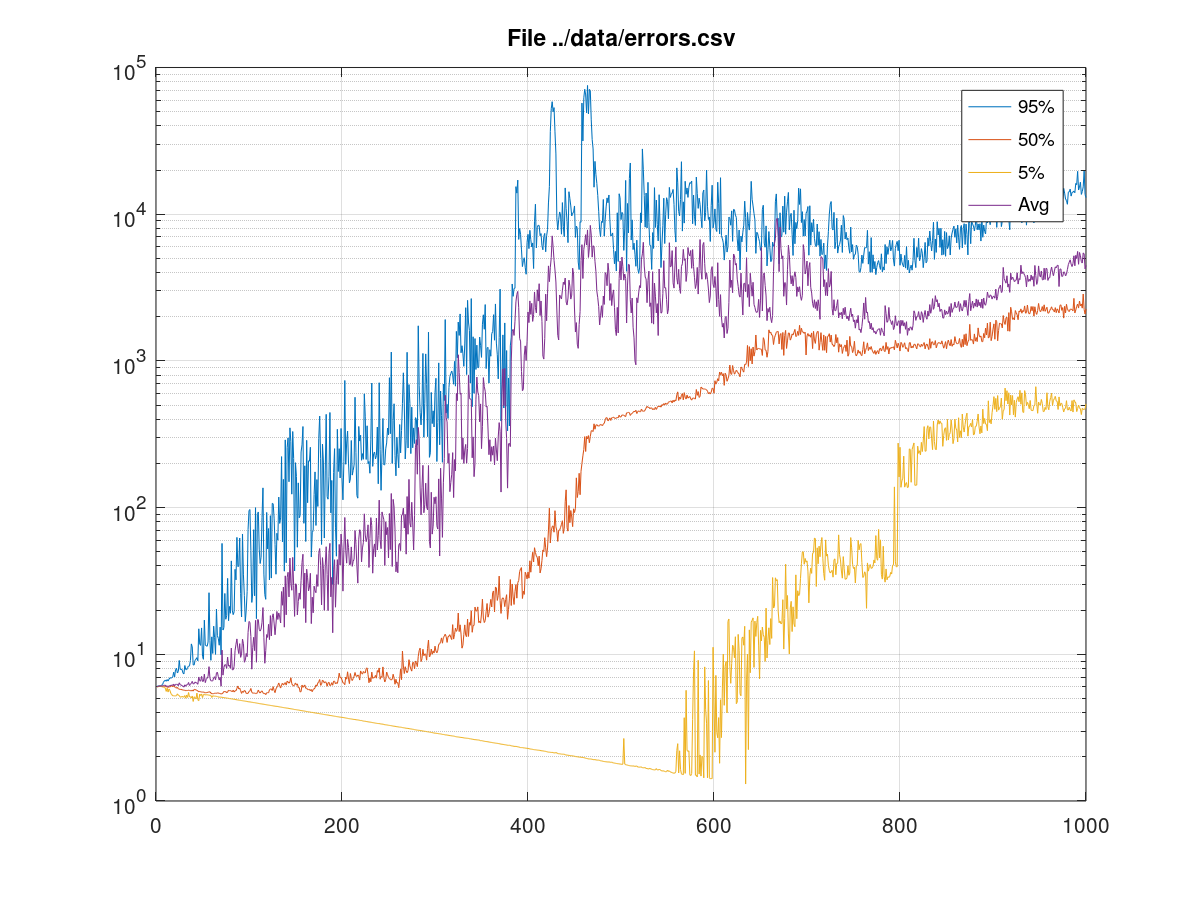
\includegraphics[width=\linewidth]{errors-07.png}
		\caption{$\lambda=0.7$.}
	\end{subfigure}
	\caption{Errors}
	\label{fig:errors}
\end{figure}
\end{document}